Similar to the \emph{loop bound} computation,
we first compute two abstract states for each simple transition path w.r.t. every level of its outer loops,
$\lpinit(\rprog, \tpath, c)$, and $\lpnext(\rprog, \tpath, c)$ based on the refined program below.
\begin{defn}[Loop Abstract States]
\label{def:alg-loopabsstate}
For a program $c$ with its refined program $\rprog_c$, a $\tpath$ and a loop $\rprog$ in $\rprog_c$ where $\tpath$ is located, we compute 
$\lpinit(\rprog, \tpath, c)$ and $\lpnext(\rprog, \tpath, c)$
w.r.t. the ranking functions as follows.
 \begin{itemize}%
 \item 
The loop initial state 
$\lpinit(\rprog, \tpath, c) \in \scexpr(c)$ computes a symbolic expression, which is an upper bound for the initial value of $\tpath$'s ranking function before
any visit of $\tpath$ and during the first execution of $\rprog$.
\[
 \begin{array}{l}
 \lpinit(\rprog, \tpath, c) \triangleq 
 \arg\max_{l_1}
 \\
 \left\{
 \varinvar(y, c) + v ~\middle\vert~ 
 \begin{array}{l} 
 (l_1, x' \leq y + v, l_2) \in \reset(x, c) 
 \\
 \land \absinit(\rprog) \leq l_1 \leq \absinit(\tpath)
 \land
 x \in \left\{ \locbound(\absevent, c) | \absevent \in \tpath \right\}
 \end{array}
 \right\}
 \end{array}
 \]
\item
The loop next state 
$\lpnext(\rprog, \tpath, c) \in \scexpr(c)$ 
estimates the amount for $\tpath$'s ranking function
that is modified before
the second visit of $\tpath$ but during the second execution of $\rprog$.
$ 
\lpnext(\rprog, \tpath, c) \triangleq 
\max\limits_{x \in \left\{ \locbound(\absevent, c) | \absevent \in \tpath \right\}}
$
%
{\small
\[
 \begin{array}{l}
 % \lpnext(\rprog, \tpath, c) \triangleq 
 % \max\limits_{x \in \left\{ \locbound(\absevent, c) | \absevent \in \tpath \right\}}
 % \\
 \left\{
 \begin{array}{l}
 \sum\limits_{\absevent \in \inc(x, c) }
 \left\{ 
 v ~\middle\vert~ \absevent = (l', x' \leq x + v, \_) \land l' \in \rprog 
 \land l' \notin \tpath \right\}
 \\ \qquad 
 + \arg\max\limits_{l_2 }
 \left\{ \varinvar(y, c) + v ~\middle\vert~ 
 (l_1, x' \leq y + v, l_2) \in \reset(x, c) \land l_1 \in \rprog \land l_1 \notin \tpath\right\}
 \\ \qquad 
 - \sum\limits_{ \absevent \in \dec(x, c) }\left\{ 
 v 
 ~\middle\vert~ \absevent = (l', x' \leq x + v, \_) \land l' \in \rprog \land l' \notin \tpath \right\}
 \\ \qquad 
 + BD(\kw{enclosed}(\tpath), c) \times \rfnext(\tpath, c)
 \end{array}
 \right\}
 \end{array}
 \]
 }
 \end{itemize}
\end{defn}
%
Then we compute the
\emph{loop reachability-bound} as below.
% using the two states and the $\rffinal$.
\begin{defn}[Loop Reachability-bound Computation]
 \label{def:looprb}
 Given a refined program $\rprog$ and a simple transition path $\tpath$ in this program, 
 let $\rprog_l$ be a loop program in $\rprog$,
 then $\rprog_l$'s \emph{loop reachability-bound} w.r.t. $\tpath$, $\lpchB(\rprog, \tpath, c)$
 is computed interactively with the abstract loop states as follows. 
 \[
 \lpchB(\rprog, \tpath, c) \triangleq
 \max\limits_{x = a \in \rffinal(\tpath, c)}
 \frac{\lpinit(\rprog, \tpath, c) - a }{\lpnext(\rprog, \tpath, c)}
 \]
\end{defn}
%
Definition~\ref{def:looprb} computes a sound \emph{loop reachability-bound} as in \highlight{Appendix~\ref{apdx:looprb-sound}}.
% In Figure~\ref{fig:relatedNestedWhileOdd-overview}, $\tpath_3$ has an outer loop program $\rprog_1^1$.
% We first compute $\lpinit(\rprog_1^1, \tpath_3, c) = n - m $ and $\lpnext(\rprog_1^1, \tpath_3, c) = n - m - 1$ and then derive $\lpchB(\rprog_1^1, \tpath_3, c) = 1$ as tight as expected.
%

% The algorithm based on the progress invariant in paper\cite{GulwaniJK09} computes similar quantity, but it estimates the iteration numbers of $l'$ in one iteration of $l$.

Figure~\ref{fig:relatedNestedWhileOdd-overview} has only one nested loop, so
the only interesting \emph{loop reachability-bound} is $\lpchB(\rprog_1^1, \tpath_3)$.
We compute $\lpinit(\rprog_1^1, \tpath_3, c) = n - m $, $\lpnext(\rprog_1^1, \tpath_3, c) = n - m - 1$ and then derive $\lpchB(\rprog_1^1, \tpath_3, c) = 1$ as expected.

We illustrate Figure~\ref{fig:threeWhile-overview} with three nested loops to better show the improvement of the \emph{loop reachability-bound}.
    %
    \begin{figure}
    \centering
    %
    \begin{subfigure}{.45\textwidth}
        $
        \begin{array}{l}
            N < m < n\\
            \kw{threeNestedWhile}(n, m, N) \triangleq \\
            \clabel{ \assign{i}{0} }^{0} ; \\
                L_1: \ewhile ~ \clabel{i < n}^{1} ~ \edo ~ \\
                \quad \Big(
                 \highlight{\clabel{\assign{j}{0}}^{2}} ;\\
                 L_3:  \quad \ewhile ~ \clabel{j < m}^{3} ~ \edo ~ \\
                \quad \quad \Big( \clabel{\assign{j}{j+1}}^{4};\\
                  \quad \quad \highlight{\clabel{\assign{w}{i}}^{5}};\\
                  L_6:  \quad \quad \ewhile ~ \clabel{w < N}^{6} ~ \edo ~ \\
                  \quad \quad \quad \Big( \clabel{\assign{w}{w + 1}}^{7}
                      \Big); \\
                      \quad \quad \clabel{\assign{i}{w}}^{8}
                      \Big); \\
                      \quad \clabel{\assign{i}{i+1}}^{9}
                  \Big)
            \end{array}
            $
    \caption{}
        \end{subfigure}
    \begin{subfigure}{.48\textwidth}
        \begin{centering}
            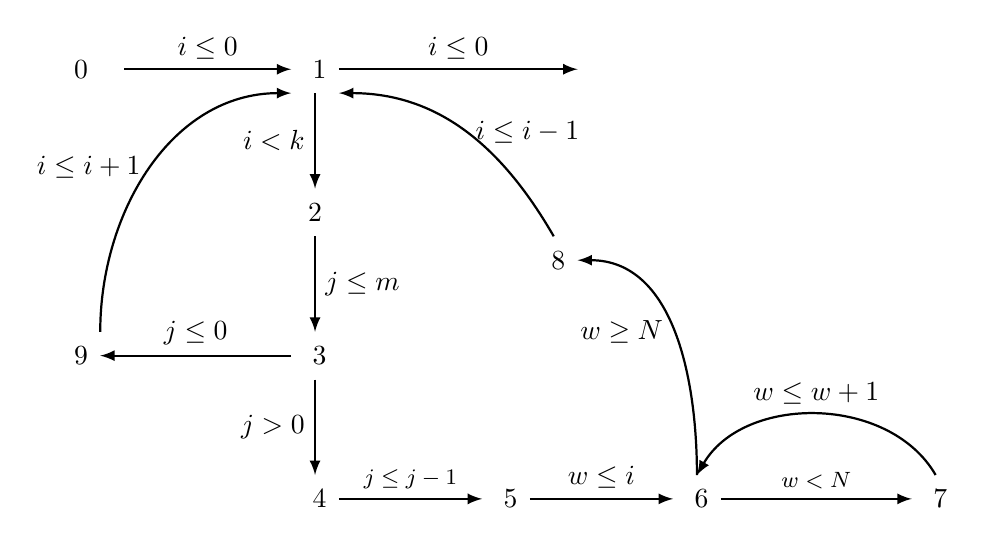
\begin{tikzpicture}[scale=\textwidth/20cm,samples=200]
                \draw[] (-5, 10) circle (0pt) node{{ $0$}};
                \draw[] (0, 10) circle (0pt) node{{ $1$}};
                \draw[] (6, 10) circle (0pt) node {{$\lex$}};
                \draw[] (0, 7) circle (0pt) node{{$2$}};
                \draw[] (0, 4) circle (0pt) node{{ $3$}};
                \draw[] (-5, 4) circle (0pt) node{{ $9$}};
                \draw[] (0, 1) circle (0pt) node{{ $4$}};
                \draw[] (4, 1) circle (0pt) node{{ $5$}};
                \draw[] (8, 1) circle (0pt) node{{ $6$}};
                \draw[] (13, 1) circle (0pt) node{{ $7$}};
                \draw[] (5, 6) circle (0pt) node{{ $8$}};
                % Counter Variables
                %
                % Control Flow Edges:
                \draw[ thick, -latex] (-4, 10)  -- node [above] {$i \leq 0$}(-0.5, 10);
                \draw[ thick, -latex] (0, 9.5)  -- node [left] {$i < k$} (0, 7.5) ;
                \draw[ thick, -latex] (0, 6.5)  -- node [right] {$j \leq m$} (0, 4.5) ;
                \draw[ thick, -latex] (0, 3.5)  -- node [left] {$j > 0$} (0, 1.5) ;
                \draw[ thick, -latex] (-0.5, 4)  -- node [above] {$j \leq 0$} (-4.5, 4) ;
                \draw[ thick, -latex] (-4.5, 4.5)  to  [out=90,in=180]  node [left] {$i \leq i + 1$ }(-0.5, 9.5);
                \draw[ thick, -latex] (0.5, 10)  -- node [above] {$i \leq 0$}  (5.5, 10);
                \draw[ thick, -latex] (0.5, 1)  -- node [above] {{\footnotesize $j \leq j - 1$}}  (3.5, 1);
                \draw[ thick, -latex] (4.5, 1)  -- node [above] {$w \leq i$}  (7.5, 1);
                \draw[ thick, -latex] (8.5, 1)  -- node [above] {{\footnotesize $w < N$}}  (12.5, 1);
                \draw[ thick, -latex] (8, 1.5)  to [out=90,in=0] node [left] {{$w \geq N$}}  (5.5, 6);
                \draw[ thick, -latex] (13, 1.5)  to  [out=120,in=60] node [above] {$w \leq w + 1$}  (8, 1.5);
                \draw[ thick, -latex] (5, 6.5)  to  [out=120,in=0]  node [right] {$i \leq i - 1$ }(0.5, 9.5);
                \end{tikzpicture}
%     \caption{}
%     \end{centering}
%     \end{subfigure}
% \begin{subfigure}{.2\textwidth}    
% \begin{centering}
    {\small
$
    \begin{array}{ll}
        \tpath_0 = (0 \to 1)
        &
        \tpath_4 = (6 \to 8 \to 3)
        \\        
        \tpath_1 = (1 \to 2 \to 3)
        &
        \tpath_5 = (3 \to 9 \to 1)
        \\
        \tpath_2 = (3 \to 4 \to 5 \to 6)
        &
        \tpath_6 = (1 \to \lex)
        \\
        \tpath_3 = (6 \to 7 \to 6)
    \end{array}
$
$
    \begin{array}{l}
        \rprog_1 = {\rprepeat(\tpath_1; 3: {\rprepeat(\tpath_2; 6 : {\rprepeat(\tpath_3)}; \tpath_4)}; \tpath_5)}
        \\
        \rprog_3 = {\rprepeat(\tpath_2; 6 : {\rprepeat(\tpath_3)}; \tpath_4)}
    \end{array}
$
}
\caption{}
\end{centering}
\end{subfigure}
    \caption{
    (a) An example of three nested loops with related iterator variables.
    (b) The abstract transition graph, simple transition paths and loop body.}
        \label{fig:threeWhile-overview}
    \end{figure}
This example is similar to the loop $L_4$ nested in the second branch in Figure~\ref{fig:relatedNestedWhileOdd-overview}.
$w$ is reset by $j$ in command 5 and $i$ is then reset by $w$, so $L_6$ is only executed in the first iteration of loops $L_1$ and $L_3$.
% \\
Then the total iterations times are
$n + m^2 - m \times N$,
and the expected \emph{reachability-bound} for location $7$ inside the $L_6$ is $N$,
for locations $4, 5$ and $8$ between the $L_3$ and $L_6$ are $(n-N) \times (m - N)$,
and $n - N$ for locations $2$ and $9$.
% \\
The challenge here is that the locations inside the loop $L_6$ have the same
\emph{reachability-bound} as the local iteration times of $L_6$.
% , as well as our \emph{path reachability-bound}.
While for the locations between $L_3$ and $L_6$, their bounds are the product of the inner and outer loop iteration bounds.
To compute the precise bound, it is critical to know
the numbers of iterations of the outer loops $L_3$ and $L_1$ such that,
during these iterations, the loop $L_6$ is ``entered'', which is exactly our \emph{loop reachability-bound}.
Figure~\ref{fig:threeWhile-overview}(a) shows its abstract transition graph,
and we compute its refined program in the bottom. 
$\rprog_1$, $\rprog_3$ and $\rprog_6$ denote the body of the loop $L_1$, $L_3$ and $L_6$ respectively.
We first compute the $\outinB(\rprog_6, \tpath_3, c) = N $ for $\tpath_3$ w.r.t. its innermost loop.
Then for its two outer loops, $L_1$ and $L_3$,
% it is nested.
we compute $\lpinit( \rprog_1, \tpath_3, c) = 0$,
$\lpnext( \rprog_1, \tpath_3, c) = N + 1 $, and
$\rffinal(\rprog_1, c) = \{ i = n, k = N \}$ and obtain
$\lpchB(\rprog_1, \tpath_3, c) = \max\{ \frac{n - 0}{n - N - 1}, \frac{N - 0}{N + 1}\} = 1$, as expected.
In the same way, we also compute $\lpchB(\rprog_3, \tpath_3, c) = 1$.

